\section{商流形}
\label{sec:lie-quotients}

前面几节反复遇到“多种记录代表同一对象”：$q$与$-q$表示同一个旋转；图~\ref{fig:lie-sphere-cosets}中一整圈旋转把$\bm e_3$送到同一个点；一个观测只确定方向时，$(2,1)^\top$与$(4,2)^\top$应视为同一对象；同一个子空间可以用许多组基张成。这些冗余都来自一个群作用：它作用在记录上，而不改变所表示的对象。把同一轨道中的记录合并，就得到真正要研究的对象集合。

第~\ref{chap:topological-spaces}章为等价关系的商集合规定了商拓扑：设$q:M\to M/G$把每个点送到所在的轨道，商中的子集$U$为开集，当且仅当$q^{-1}(U)$在$M$中为开集。本节要进一步回答：什么时候这个商还能带上光滑结构，使后面几章的切空间、微分与度量都能使用。任意群作用的商一般做不到这一点。

\subsection{光滑商的条件}
\label{sec:lie-smooth-quotient-conditions}

先看两个商不是流形的例子，从中读出群作用需要满足的条件，再陈述这些条件下的商流形定理，并用闭子群构造最常用的一类商。

\paragraph{两类失败}
第一类失败来自稳定子不一致。第~\ref{sec:lie-orbits-stabilizers}节中，$\mathrm{SO}(2)$作用于$\mathbb R^2$的商是$[0,\infty)$。非零点的轨道是圆，稳定子平凡；原点的轨道是一个点，稳定子是整个群。商在$0$处有一个端点，那里的任何邻域都不同胚于开区间，所以商不是无边界的一维流形，见图~\ref{fig:lie-quotient-failures}(a)(b)。不能只因为“去掉了一个旋转自由度”就宣布商是$2-1=1$维流形。

第二类失败来自轨道挤在一起。取无理数$\alpha$，让整数加法群$\mathbb Z$按$k\cdot\bm x=\bm R(2\pi k\alpha)\bm x$作用在单位圆上。$k\neq0$时$k\alpha$不是整数，没有点被固定，稳定子都是平凡的。但每条轨道都在圆上稠密。

下面证明这一点。把圆分成$N$段长为$2\pi/N$的弧，同一条轨道上$k=0,1,\ldots,N$这$N+1$个点必有两个落在同一段，设为$k_1<k_2$。令$k=k_2-k_1$，则转角$2\pi k\alpha$模$2\pi$后绝对值小于$2\pi/N$，且不为零。反复施加这个小旋转，轨道上就出现间距小于$2\pi/N$的点，$N$可以任意大，所以轨道稠密。

\begin{BookInlineFigure}
  \centering
  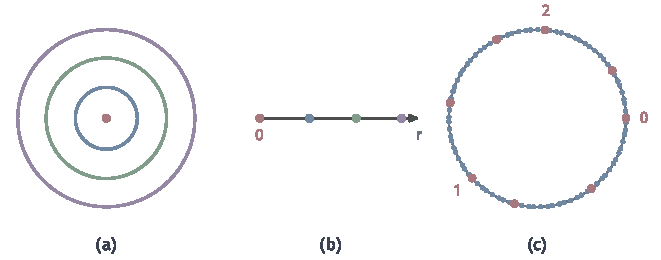
\includegraphics[width=112mm]{figures/04-spaces-measures-and-geometry/04-manifolds/matplotlib/lie-quotient-failures/figure.pdf}
  \caption{商不是流形的两种情形。(a)$\mathrm{SO}(2)$作用于平面的轨道：同心圆与中心的原点。(b)轨道空间$[0,\infty)$，用半径编号，同色的点对应同色的圆，原点（红）对应端点。(c)无理旋转的一条轨道，$\alpha=(\sqrt5-1)/2$，大红点依次是前$8$个点$k=0,\ldots,7$，小蓝点是$k=8,\ldots,89$，已经密布整个圆。}
  \label{fig:lie-quotient-failures}
\end{BookInlineFigure}

于是商空间的拓扑很差。设$U$是商中的非空开集，它的原像是圆上的非空开集，且由整条轨道组成。任何一条轨道都稠密，所以都与这个开集相交，从而整条轨道都在其中，$U$就是整个商。商的开集只有空集和全集，不同的点不能被开集分开，它不是Hausdorff空间，更不是流形。

\paragraph{自由与适当}
这两类失败分别对应下面两个条件。

\begin{definition}[自由作用与适当作用]
\label{def:lie-free-proper-action}
设Lie群$G$光滑地作用于流形$M$，即$G\times M\to M$是光滑映射。若每个点的稳定子都只含单位元，就称作用是\term{自由作用}（free action）。若映射$G\times M\to M\times M$，$(g,x)\mapsto(g\cdot x,x)$下每个紧集的原像都是紧集，就称作用是\term{适当作用}（proper action）。
\end{definition}

自由性排除了第一类失败：各点的稳定子相同，轨道的维数处处等于群的维数。适当性排除了第二类失败：它禁止群中“跑到无穷远”的元素把一个点又带回原处附近，从而使不同的轨道能被邻域分开。

紧Lie群的光滑作用总是适当的，有限群作为零维Lie群也是如此。上面的$\mathbb Z$作用不适当：取$\bm x$的一个邻域，无穷多个$k$把$\bm x$送回这个邻域，这些$k$组成无界的集合。下面的定理说明，这两个条件足以得到光滑的商。

\begin{theorem}[商流形定理]
\label{thm:lie-quotient-manifold}
设Lie群$G$在$m$维光滑流形$M$上的光滑作用既自由又适当，$G$的维数为$k$。则轨道空间$M/G$在商拓扑下是$m-k$维的拓扑流形，并且具有唯一的光滑结构，使商映射$q:M\to M/G$是光滑淹没。
\end{theorem}

定理的证明需要构造横截于轨道的局部切片，并用常秩定理验证转移映射光滑，篇幅较长，读者可查阅\scite{math-lee2013smooth}。证明的思路是：在每个点附近，取与轨道横截的一小片子流形，由自由与适当两个条件，每条附近的轨道与这片子流形恰好相交一次，这片子流形就充当商的坐标图。

所得的光滑结构称为\term{商流形}（quotient manifold）。由$q$是淹没，$M/G$上的映射$f$光滑，当且仅当$f\circ q$在$M$上光滑。第~\ref{sec:lie-invariant-equivariant}节中经由轨道分解的不变映射，正是用这种方式落到商上。

定理给的是充分条件，不是唯一可用的情形。对没有给定作用的一般等价关系，商可能根本不是流形；即使作用存在，也要逐项核对光滑、自由与适当，不能把任意等价关系的商都当作光滑流形。

\paragraph{齐性空间}
最常用的一类商来自闭子群。设$H$是Lie群$G$的闭子群，它按$h\cdot g=gh^{-1}$作用在$G$上，轨道恰是左陪集$gH$。这个作用自由，并且可以证明是适当的（闭性保证陪集不会挤在一起），所以$G/H$是$\dim G-\dim H$维的流形，称为\term{齐性空间}（homogeneous space）。它之所以“齐性”，是因为$G$按$g'\cdot(gH)=(g'g)H$传递地作用在$G/H$上，任何两点之间都有一个变换相连。

齐性空间常常就是某个熟悉的空间。若$G$光滑且传递地作用于流形$X$，$x_0\in X$的稳定子为$H$，由定理~\ref{thm:lie-orbit-stabilizer}，$gH\mapsto g\cdot x_0$是从$G/H$到$X$的双射，并且可以进一步证明它是微分同胚。以$\mathrm{SO}(3)$作用于$S^2$为例，$\bm e_3$的稳定子是绕第三轴的旋转，与$\mathrm{SO}(2)$同构，所以
\begin{equation}
 \mathrm{SO}(3)/\mathrm{SO}(2)\cong S^2,\qquad \bm R\,\mathrm{SO}(2)\mapsto\bm R\bm e_3.
 \label{eq:lie-so3-so2}
\end{equation}

维数核对：$3-1=2$。图~\ref{fig:lie-sphere-cosets}(b)画的正是这个商的一条纤维：$\bm R$的第三列决定了陪集，前两列在切平面内还可以任意转动，这一转动正是被商掉的自由度。

另一个例子回到四元数。有限群$\{(1,\bm0),(-1,\bm0)\}$按左乘作用在$S^3$上，没有不动点，作用自由且适当，商$S^3/\{\pm1\}$是三维流形。由定理~\ref{thm:lie-double-cover}，$q\mapsto\bm R(q)$在每条轨道$\{q,-q\}$上取同一个值，并且不同的轨道给出不同的旋转，于是它在商上给出$S^3/\{\pm1\}$到$\mathrm{SO}(3)$的双射；结合它是局部微分同胚，可知这个双射是微分同胚。

\subsection{射影空间}
\label{sec:lie-projective-space}

相机把空间中的一点投影到成像平面时，只能确定这一点所在的视线方向，不能确定它沿视线有多远。若把视线用一个非零向量记录，那么$\bm x$与$\lambda\bm x$（$\lambda\neq0$）记录的是同一条视线。忽略这种非零倍数，就得到射影空间。

\begin{definition}[实射影空间]
\label{def:lie-projective-space}
非零实数在乘法下构成群$\mathbb R^*=\mathbb R\setminus\{0\}$，它按$\lambda\cdot\bm x=\lambda\bm x$作用于$\mathbb R^{n+1}\setminus\{\bm0\}$。轨道空间
\begin{equation}
 \mathbb{RP}^n=(\mathbb R^{n+1}\setminus\{\bm0\})/\mathbb R^*
 \label{eq:lie-rpn}
\end{equation}
称为$n$维\term{实射影空间}（real projective space）。$\bm x$所在的轨道记为$[\bm x]=[x_1:\cdots:x_{n+1}]$，称为\term{齐次坐标}（homogeneous coordinates）。
\end{definition}

$\mathbb{RP}^n$的一个点就是$\mathbb R^{n+1}$中过原点的一条直线。零向量必须除去：它的所有倍数都是零，不表示任何方向。这个作用是自由的，因为$\lambda\bm x=\bm x$与$\bm x\neq\bm0$推出$\lambda=1$。

作用也是适当的。设$K$是$(\mathbb R^{n+1}\setminus\{\bm0\})^2$中的紧集，$K$的两个分量的范数都落在某个区间$[a,b]$内，$a>0$。若$(\lambda\bm x,\bm x)\in K$，则
\[
\lvert\lambda\rvert=\frac{\lVert\lambda\bm x\rVert_2}{\lVert\bm x\rVert_2}\in\Bigl[\frac ab,\frac ba\Bigr].
\]
所以原像中的$\lambda$在$\mathbb R^*$的紧子集内，$\bm x$在$K$的投影内，原像又是闭集，从而是紧集。由定理~\ref{thm:lie-quotient-manifold}，$\mathbb{RP}^n$是$n$维光滑流形，维数核对$(n+1)-1=n$。把代表元缩放到单位球面，只剩符号自由度，于是它也可以写成$S^n/\{\pm1\}$。

\paragraph{仿射图与无穷远点}
商流形的坐标可以直接写出来。在$x_j\neq0$的点上，每个类都唯一地有一个代表使第$j$个分量为$1$，于是令
\[
U_j=\{[\bm x]:x_j\neq0\},\qquad
\varphi_j([\bm x])=\Bigl(\frac{x_i}{x_j}\Bigr)_{i\neq j}\in\mathbb R^n .
\]
$\varphi_j$不依赖代表元，因为分子分母同乘$\lambda$。$U_j$的原像$\{x_j\neq0\}$是开集，所以$U_j$是开集。$\varphi_j\circ q$是有理函数，因而连续；逆映射把$\bm u$送到第$j$分量为$1$的向量再取类，也连续，所以$\varphi_j$是同胚。两张图的重叠处，坐标转换是分量之比，分母非零，因而光滑。这些图称为\term{仿射图}（affine chart），$n+1$张就覆盖了$\mathbb{RP}^n$。

相对于一张选定的仿射图$U_{n+1}$，不在其中的点$\{x_{n+1}=0\}$称为\term{无穷远点}（point at infinity）。它们不是向坐标中加入数值$\infty$，而是这张图未覆盖、在其他图中可以正常记录的点。

看$\mathbb{RP}^1$的例子。末分量图中，每条不水平的直线与直线$x_2=1$恰好相交一次，交点的第一坐标$x_1/x_2$就是这条直线的坐标，见图~\ref{fig:lie-projective}(a)。例如$[2:4]=[1:2]$的坐标是$\frac12$。水平线$[1:0]$与$x_2=1$不相交，它不在这张图中，但在首分量图中坐标为$0$。所以$\mathbb{RP}^1$是一条直线加上一个无穷远点，拓扑上是一个圆。

\begin{BookInlineFigure}
  \centering
  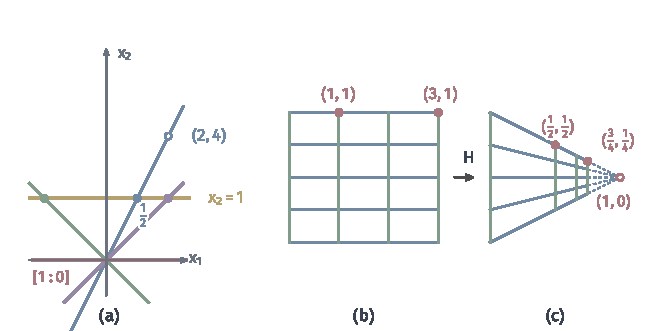
\includegraphics[width=112mm]{figures/04-spaces-measures-and-geometry/04-manifolds/matplotlib/lie-projective/figure.pdf}
  \caption{射影空间的仿射图与射影变换。(a)$\mathbb{RP}^1$的末分量图：过原点的直线与黄线$x_2=1$的交点给出坐标，蓝线是$[2:4]$，坐标为$\frac12$；红色水平线$[1:0]$不与黄线相交，是这张图的无穷远点。(b)平面上的方格，蓝线$v=$常数，绿线$u=$常数，红点是$(1,1)$与$(3,1)$。(c)方格在$\bm H$下的像（横向比例放大）：绿线仍是竖线，蓝线不再平行，延长后交于$(1,0)$。}
  \label{fig:lie-projective}
\end{BookInlineFigure}

在射影平面$\mathbb{RP}^2$中，非零系数向量$\bm\ell\in\mathbb R^3$确定直线$\{[\bm x]:\bm\ell^\top\bm x=0\}$，$\bm\ell$与它的非零倍数确定同一条直线。在$x_3=1$的图中它就是$\ell_1u+\ell_2v+\ell_3=0$。

两条平行线$u=0$与$u=1$的系数分别是$(1,0,0)^\top$与$(1,0,-1)^\top$。同时满足两个方程，第一个方程给出$x_1=0$，第二个方程再给出$x_3=0$，所以交点的齐次坐标是$[0:1:0]$，在这张图之外。平行线在射影平面中交于一个无穷远点。

\paragraph{射影变换}
可逆线性映射把过原点的直线映成过原点的直线，所以诱导出射影空间上的变换。

\begin{definition}[射影变换]
\label{def:lie-projective-transformation}
对$\bm H\in\mathrm{GL}(n+1,\mathbb R)$，映射$[\bm x]\mapsto[\bm H\bm x]$称为$\mathbb{RP}^n$上的\term{射影变换}（projective transformation）。
\end{definition}

它不依赖代表元，因为$\bm H(\lambda\bm x)=\lambda\bm H\bm x$；$\bm H\bm x\neq\bm0$由$\bm H$可逆保证。在仿射图中它是有理函数，因而光滑，逆变换由$\bm H^{-1}$给出，所以是微分同胚。$\bm H$与$c\bm H$（$c\neq0$）给出同一个变换，所以射影变换组成的群是$\mathrm{GL}(n+1,\mathbb R)$按非零数量矩阵取商，参数个数为$(n+1)^2-1$，平面的情形$n=2$有$8$个自由度。

射影变换保持点在线上的关系。若点按$\bm x'=\bm H\bm x$变换，令直线系数按$\bm\ell'=\bm H^{-\top}\bm\ell$变换，则
\[
\bm\ell'^\top\bm x'=\bm\ell^\top\bm H^{-1}\bm H\bm x=\bm\ell^\top\bm x,
\]
所以$\bm x$在$\bm\ell$上当且仅当$\bm x'$在$\bm\ell'$上。

它一般不保持长度、角度和平行。例如
\[
\bm H=\begin{bmatrix}1&0&0\\0&1&0\\1&0&1\end{bmatrix},\qquad
(u,v)\longmapsto\Bigl(\frac{u}{u+1},\frac{v}{u+1}\Bigr)\quad(u\neq-1).
\]
点$(1,1)$变成$(\frac12,\frac12)$，点$(3,1)$变成$(\frac34,\frac14)$。

这两个像点的连线延长后经过$(1,0)$，因为直线$v=1$上的点都是$\frac{v}{u+1}=\frac1{u+1}=1-\frac{u}{u+1}$，满足$v'=1-u'$。所有水平线$v=c$的像都经过$(1,0)$，图~\ref{fig:lie-projective}(b)(c)中平行的蓝线在像中汇聚到这一点。这个点是平行线在无穷远处交点的像：$\bm H(1,0,0)^\top=(1,0,1)^\top$。

直线$u=-1$上的点仍有合法的齐次像，只是像的第三分量为零，落到末分量图的无穷远处。所以“除以末分量”只能在它非零时进行，不能当作全局的线性运算。

刚体变换是射影变换的特例：式~\eqref{eq:lie-homogeneous-pose}中的$\bm T$底行为$(0,0,0,1)$，把末分量为$1$的点仍送到末分量为$1$的点，保持无穷远点组成的集合。由给定的点对应估计一个未知的$\bm H$，需要消去未知的比例并处理退化配置，这是第~\ref{chap:spatial-map-estimation}章的问题。

\subsection{Grassmann空间}
\label{sec:lie-grassmann}

射影空间研究$\mathbb R^{n+1}$中的一维子空间。数据分析中常常关心更高维的子空间，例如一组样本主要分布在哪个$k$维子空间附近。子空间本身是一个几何对象，但要计算它，通常得选一组基，把它记为矩阵；不同的基给出同一个子空间。

\paragraph{用基表示子空间}
设$\bm Y\in\mathbb R^{n\times k}$的列线性无关，它的列空间是一个$k$维子空间。若$\bm A\in\mathrm{GL}(k,\mathbb R)$，则$\bm Y\bm A$的各列是$\bm Y$各列的线性组合，并且仍线性无关，所以列空间不变。反过来，若$\bm Y,\bm Y'$列空间相同，则$\bm Y'$的每一列都能唯一地写成$\bm Y$各列的组合，即$\bm Y'=\bm Y\bm A$，且$\bm A$可逆。所以“同一子空间”恰好是$\mathrm{GL}(k,\mathbb R)$按右乘作用的轨道，这个对象因此可以用商来定义。

\begin{definition}[Grassmann空间]
\label{def:lie-grassmann}
$\mathbb R^n$中全体$k$维线性子空间组成的集合记为$\mathrm{Gr}(k,n)$，称为\term{Grassmann空间}（Grassmannian）。
\end{definition}

列满秩的$n\times k$矩阵组成$\mathbb R^{n\times k}$中的开集，记为$F$，$\mathrm{GL}(k,\mathbb R)$按$\bm A\cdot\bm Y=\bm Y\bm A^{-1}$在其上作用。作用是自由的：$\bm Y\bm A=\bm Y$与列满秩推出$\bm A=\bm I$。

作用也是适当的。设$K\subset F\times F$紧，若$(\bm Y\bm A^{-1},\bm Y)\in K$，记$\bm Y'=\bm Y\bm A^{-1}$，由列满秩解出
\[
\bm A=(\bm Y'^\top\bm Y')^{-1}\bm Y'^\top\bm Y,\qquad
\bm A^{-1}=(\bm Y^\top\bm Y)^{-1}\bm Y^\top\bm Y'.
\]
两个公式的右边在紧集$K$上连续，所以$\bm A$与$\bm A^{-1}$都有界，原像落在$\mathrm{GL}(k,\mathbb R)$的紧子集与$K$的投影之积内，又是闭集，从而是紧集。

由定理~\ref{thm:lie-quotient-manifold}，$\mathrm{Gr}(k,n)$是光滑流形，维数为$nk-k^2=k(n-k)$。$k=1$时它就是$\mathbb{RP}^{n-1}$，维数$n-1$。

\paragraph{用标准正交基表示}
计算中更常用标准正交基。满足$\bm Y^\top\bm Y=\bm I_k$的$n\times k$矩阵全体称为\term{Stiefel流形}（Stiefel manifold），记为$\mathrm{St}(k,n)$。与定理~\ref{thm:lie-orthogonal-group-manifold}的证明相同，约束$\bm Y^\top\bm Y=\bm I_k$取值于$\mathrm{Sym}(k)$且以$\bm I_k$为正则值，所以$\mathrm{St}(k,n)$的维数是$nk-k(k+1)/2$。

同一子空间的两组标准正交基只差一个正交矩阵，$\bm Y'=\bm Y\bm Q$，$\bm Q\in\mathrm O(k)$。紧群$\mathrm O(k)$的这一作用自由且适当，于是
\begin{equation}
 \mathrm{Gr}(k,n)\cong\mathrm{St}(k,n)/\mathrm O(k).
 \label{eq:lie-grassmann-stiefel}
\end{equation}
维数核对：
\[
nk-\frac{k(k+1)}2-\frac{k(k-1)}2=k(n-k),
\]
与上一段的结果一致。$k=n$时$\mathrm{St}(n,n)=\mathrm O(n)$，$\mathrm{Gr}(n,n)$只有一个点。

\paragraph{子空间与标架的区别}
标准正交基$\bm Y$称为一个标架，它比子空间多记录了$k(k-1)/2$个自由度，即在子空间内部怎样选取各轴。图~\ref{fig:lie-grassmann-frames}(a)中$\mathbb R^3$的一张平面对应两组不同的标架，它们是$\mathrm{St}(2,3)$中两个不同的点，却是$\mathrm{Gr}(2,3)$中同一个点。

消除这些自由度的一种方式是改用正交投影矩阵$\bm P=\bm Y\bm Y^\top$。对$\bm Q\in\mathrm O(k)$，
\[
(\bm Y\bm Q)(\bm Y\bm Q)^\top=\bm Y\bm Q\bm Q^\top\bm Y^\top=\bm Y\bm Y^\top,
\]
所以$\bm P$只依赖子空间；反过来，$\bm P$的列空间就是该子空间。于是$\mathrm{Gr}(k,n)$可以与秩为$k$的对称幂等矩阵一一对应，这个矩阵集合是
\[
\{\bm P:\bm P^\top=\bm P,\ \bm P^2=\bm P,\ \operatorname{tr}\bm P=k\}.
\]

切方向也要区分。在标架$\bm Y$处，Stiefel流形的切向量$\bm\Delta$满足$\bm Y^\top\bm\Delta+\bm\Delta^\top\bm Y=\bm0$。设$\bm Y_\perp$的列是正交补的一组标准正交基，切向量分解为
\[
\bm\Delta=\bm Y\bm\Omega+\bm Y_\perp\bm B,\qquad \bm\Omega^\top=-\bm\Omega .
\]

形如$\bm Y\bm\Omega$的方向只在子空间内部转动标架，不改变子空间，称为竖直方向；形如$\bm Y_\perp\bm B$（满足$\bm Y^\top\bm\Delta=\bm0$）的方向才真正把子空间推向别处，称为水平方向。水平方向组成的线性空间维数为$(n-k)k$，恰好是$\mathrm{Gr}(k,n)$的维数，可以作为子空间处切空间的具体表示。

取$n=3$，$k=2$，$\bm Y=[\bm e_1,\bm e_2]$。竖直方向和水平方向各取一个例子：
\[
\bm\Delta_v=[\bm e_2,\ -\bm e_1],\qquad
\bm\Delta_h=[\tfrac12\bm e_3,\ \bm0].
\]
前者对应$\bm\Omega=\begin{bmatrix}0&-1\\1&0\end{bmatrix}$，后者对应$\bm B=(\tfrac12,0)$，它把平面绕$\bm e_2$轴倾斜。图~\ref{fig:lie-grassmann-frames}(b)画出了这两种方向。

\begin{BookInlineFigure}
  \centering
  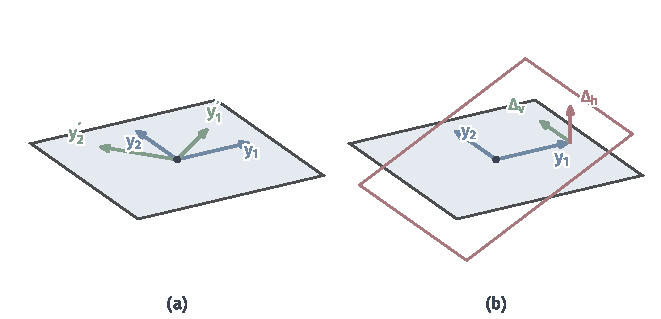
\includegraphics[width=112mm]{figures/04-spaces-measures-and-geometry/04-manifolds/matplotlib/lie-grassmann-frames/figure.pdf}
  \caption{$\mathbb R^3$中的平面与标架。(a)同一张平面的两组标准正交基，蓝色$\bm Y$与绿色$\bm Y\bm Q$相差平面内转动$38^\circ$，它们是$\mathrm{St}(2,3)$的两个点、$\mathrm{Gr}(2,3)$的同一个点。(b)标架$\bm Y=[\bm e_1,\bm e_2]$处的两种切向量。绿箭头是竖直方向$\bm\Delta_v$的第一列（画成$0.75$倍长），只转动标架；红箭头是水平方向$\bm\Delta_h$的第一列，把平面倾斜到红框所示的新平面。}
  \label{fig:lie-grassmann-frames}
\end{BookInlineFigure}

\paragraph{局部坐标}
子空间也有类似仿射图的坐标。若一个$k$维子空间与后$n-k$个坐标组成的子空间只交于零，它就有唯一的一组基写成$\begin{bmatrix}\bm I_k\\\bm B\end{bmatrix}$，$\bm B\in\mathbb R^{(n-k)\times k}$。$\bm B$的$k(n-k)$个元素就是这类子空间的坐标。$k=1$时它正是射影空间的首分量仿射图。不满足这个条件的子空间，换一组$k$个坐标的位置即可同样处理。

以正交约束或子空间为未知量的优化，要把这里的切方向、商结构与回到流形的更新方式结合起来，这是\BookChapterRef{chap:manifold-optimization}{卷五第25章“流形优化”}的内容；本节只说明这些未知量是什么对象、有多少自由度。
